\documentclass[letterpaper, 11pt]{article}
\usepackage{amsmath}
\usepackage{mathtools}
\usepackage{amssymb}
\usepackage{float}
\usepackage{inputenc}
\usepackage[left=2cm, right=2cm, top=2cm, bottom=2cm]{geometry}
\usepackage{graphicx}
\usepackage{float}
\usepackage{caption}
\usepackage{extarrows}
\usepackage{xcolor}
\usepackage{lscape}
\usepackage{pdflscape}
\usepackage{pdfpages}
\usepackage{multicol}
\usepackage{leftindex}
\usepackage{fancybox,framed}
\usepackage{algorithm2e}
\usepackage{indentfirst}
\SetKwComment{Comment}{/* }{ */}
%\RestyleAlgo{ruled}
\usepackage{mathtools}
\usepackage{hyperref}
\hypersetup{
    colorlinks=false,
    }

% Listings
\usepackage{listings}
\usepackage{color}
\usepackage{xcolor}
\definecolor{mygreen}{rgb}{0,0.6,0}
\definecolor{mygray}{rgb}{0.5,0.5,0.5}
\definecolor{mymauve}{rgb}{0.58,0,0.82}

\lstset{
  backgroundcolor=\color{white},   % choose the background color; you must add \usepackage{color} or \usepackage{xcolor}; should come as last argument
  basicstyle=\small\ttfamily,        % the size of the fonts that are used for the code
  breakatwhitespace=false,         % sets if automatic breaks should only happen at whitespace
  breaklines=true,                 % sets automatic line breaking
  captionpos=t,                    % sets the caption-position to bottom
  commentstyle=\color{mygreen},    % comment style
  deletekeywords={...},            % if you want to delete keywords from the given language
  escapeinside={\%*}{*)},          % if you want to add LaTeX within your code
  extendedchars=true,              % lets you use non-ASCII characters; for 8-bits encodings only, does not work with UTF-8
  firstnumber=1,                % start line enumeration with line 1000
  frame=false,	                   % adds a frame around the code
  keepspaces=true,                 % keeps spaces in text, useful for keeping indentation of code (possibly needs columns=flexible)
  keywordstyle=\color{blue},       % keyword style
  language=Python,                 % the language of the code
  morekeywords={*,...},            % if you want to add more keywords to the set
  numbers=none,                    % where to put the line-numbers; possible values are (none, left, right)
  numbersep=5pt,                   % how far the line-numbers are from the code
  numberstyle=\tiny\color{mygray}, % the style that is used for the line-numbers
  rulecolor=\color{black},         % if not set, the frame-color may be changed on line-breaks within not-black text (e.g. comments (green here))
  showspaces=false,                % show spaces everywhere adding particular underscores; it overrides 'showstringspaces'
  showstringspaces=false,          % underline spaces within strings only
  showtabs=false,                  % show tabs within strings adding particular underscores
  stepnumber=5,                    % the step between two line-numbers. If it's 1, each line will be numbered
  stringstyle=\color{mymauve},     % string literal style
  tabsize=4,	                   % sets default tabsize to 2 spaces
  title=\lstname                   % show the filename of files included with \lstinputlisting; also try caption instead of title
}


% NewCommands
\newcommand{\peq}{ \mathrel{+}= }
\newcommand{\muleq}{ \mathrel{*}= }
\newcommand{\sign}{ \text{sign}}
\newcommand{\bm}[1]{\begin{bmatrix} #1 \end{bmatrix}}
\newcommand{\mat}[1]{\begin{matrix} #1 \end{matrix}}
\newcommand{\lx}[2]{\leftindex #1 {#2}}
\newcommand{\norm}[1]{\left\lvert #1 \right\rvert}
\newcommand{\itbf}[1]{\textit{\textbf{#1}}}
\newcommand{\mdet}[1]{\norm{\begin{matrix} #1 \end{matrix}}}
\newcommand{\pbox}[1]{\fbox{\begin{minipage}{\textwidth} #1 \end{minipage}}}
\newcommand{\lstln}[1]{\lstinline|#1|}
\newcommand{\lr}[1]{\left( #1 \right)}
\newcommand{\lrb}[1]{\left[ #1 \right]}


\title{
    \begin{figure}[H]
        \centering
        
\includegraphics[width = 0.4\textwidth]{./figs/purdue-university-1-logo-png-transparent.png}
    \end{figure}
    \doublebox{CUMMINS/PURDUE STRATEGIC ALLIANCE AGREEMENT}
}
\date{}

\begin{document}
\maketitle
\tableofcontents
\begin{center}
    \textsc{Appendix A}\\
    \bigskip
    \textsc{Research Project Plan}\\
    \textbf{Cummins Proposal Worksheet}
\end{center}
\tableofcontents

\bigskip

\textbf{Title:} On-board diagnostics (OBD) tool development for
catalyst-degradation in automotive Selective Catalytic Reduction (SCR)
systems.\\

\textbf{Date} \today\\

This is a Research Project Plan pursuant to the Strategic Alliance Agreement
(“Agreement”) executed on August 13, 2019,  between Cummins Inc. and Purdue
University.  Upon the party's mutual execution below, the Research Project Plan
shall be awarded and performed in accordance with the Agreement.

\section{Research Project Description}

\subsection{Objective}
To develop model-based non-intrusive on-board diagnostics (OBD) tools to detect
catalyst-degradation in automotive Selective Catalytic Reduction (SCR) - Ammonia
Slip Catalyst (ASC) system.

\subsection{Background}
Modern Diesel after-treatment systems with Selective Catalytic Reduction (SCR)
- Ammonia Slip Catalyst (ASC) need on-board diagnostics (OBD) tools that can
accurately report SCR degradation level while avoiding false pass and false
fail. The diagnostic tool's performance must contain the following features: 1)
high estimation accuracy; 2) high robustness against various noise factors
under harsh on-road operating conditions; 3) minimal negative impact on SCR
emissions control; and 4) cost-effective by using existing SCR configurations
and commercially available $NO_x$ sensors. Purdue University and Tennessee
Technological University (TTU) have researched the literature on
control-oriented SCR-aging models and various estimation methods for developing
such a diagnostic tool. Since it is very difficult to imitate real-world
catalyst degradation using test-cell accelerated aging, none of the existing
control-oriented SCR-aging models have been validated or tested on real-world
catalyst degradation data. Another limitation of existing OBD methods for SCR
systems is that they do not consider the presence of Ammonia Slip Catalyst
(ASC) in series with SCR. Also, most existing OBD approaches cannot work under
the limitations of commercial after-treatment instrumentation such as no NH3
sensors, cross-sensitive $NO_x$ sensors etc. Therefore, development of better
models to design OBD methods that can work with commercial systems under
on-road conditions is required. Purdue University and TTU have already
initiated the research effort in collaboration with Cummins Inc. to fill this
gap by investigating model-based and data-driven diagnostic algorithms to
detect aging in SCR systems. The overall research endeavor includes:

\begin{enumerate}
\item achieving insight in SCR aging from modeling and diagnostic perspectives
via the comprehensive analysis of experimental data;
\item developing accurate control-oriented after-treatment models to predict
reduced emissions' performance at different degradation levels, and
\item developing robust and effective non-intrusive diagnostic methods that could distinguish SCR catalysts at different aging levels for real-world driving conditions.
\end{enumerate}

As part of this effort, Cummins provided real-world truck data and test-cell
data, along with seed funds for the year 2022, to Purdue University and TTU. In
the year 2022, Purdue and TTU thoroughly studied the data, and explored several
model-based and data-driven OBD approaches. For the model-based approach,
Purdue developed a model and a model-based OBD for the operating conditions
when ASC is active, and TTU has been working on a complementary model for
conditions when the ASC is inactive. For the data-driven approach, Purdue
worked on a binary classifier to classify the catalyst as either degreened (DG)
or EUL at each time-stamp, and TTU has been working on exploring several
methods to detect $NO_x$-rich operating conditions which are suitable to
extract distinct features from each truck. The motivation behind this proposal
is to obtain funds for the year 2024 to continue this effort to develop OBD
method capable of meeting the previously laid out requirements.

This is a joint effort by Purdue University and TTU and this document proposes
Purdue's share of the work for 2024. Purdue will focus on improving the
model-based and data-driven OBD approaches with the following goals for 2023:
\begin{enumerate}
\item validate and improve the diagnostics-oriented SCR-ASC model using
additional test-cell data and a high-fidelity SCR-ASC model from Cummins' (AVL
boost model)
\item validate and improve both model-based and data-driven OBD methods using
high-fidelity simulations and truck data with known aging levels (could be DG
and/or EUL), and
\item  support TTU in development and demonstration of model-based and data-driven OBD methods that rely on detecting $NO_x$-rich operating conditions where ASC is inactive
\end{enumerate}

Based on the findings from data analysis, models and diagnostic algorithms
developed in 2022 and 2023 by Purdue and TTU, the implementation and field
validation of model-based non-intrusive diagnostic methods that could work with
the Cummins existing commercial SCR systems will be planned in follow-on work.

\subsection{Research Expertise and Qualification}
The research team consists of Purdue University and TTU. The research expertise and qualification of Purdue University to successfully complete the project are described as follows:

The research group from Purdue University is led by Prof. Peter H. Meckl. Prof.
Meckl is a Professor of Mechanical Engineering at Purdue University. He received
his B.S. degree in Mechanical Engineering from Northwestern University in 1981,
M.S. in Mechanical Engineering from MIT in 1984, and Ph.D. in Mechanical
Engineering from MIT in 1988. He was the principal investigator for Purdue
EcoCAR2 project. He and his team have written 45 archival journal papers and
over 100 refereed conference papers, many of them concerning automotive control.
Much of the research on engine and after-treatment diagnostics and control has
been sponsored by Cummins, work that spans over 25 years. He has been involved
in research on modeling and control of urea-SCR systems starting in 2013 and has
graduated four M.S. thesis students who worked on modeling, estimation, and
control for the urea-SCR system. He has one PhD student currently
working on developing OBD for urea-SCR systems.



\subsection{Summary of work and results from 2023}

\subsubsection{Conclusions}
The full non-linear model for gas concentrations was derived based on a CSTR
model with reduced-order dynamics, that were previously justified. Model
parameters were determined as explicit functions of reaction rates and the
catalyst's ammonia storage capacity.  Parameter identification, beginning with
the output equation and focusing on $NO_x$ sensor cross-sensitivity ($\chi$),
was carried out using RMC test-cell data from degreened and aged catalysts. A
preliminary indicator of aging was observed from the catalyst's storage capacity
versus temperature curve.

\newpage
\section{Summary of work and results from 2023}

%===============================================================================
%===============================================================================
\subsection{Nonlinear Model: Effects on Parametrization from State Choice}

\subsubsection{Reaction Rates}
\itbf{Assumptions:}
\begin{enumerate}
\item The reaction rates are only functions of gas-phase concentrations of $NO$,
$NH_3$, the adsorbed Ammonia and the available adsorption sites.

\item The concentration rates are converted into molar-rate so that the
mass balance in control volume approach (CSTR) can be performed. For gaseous reactants:
$$ M_g = C_g V \implies R_i = V r_i $$
The number of moles of the adsorbent is directly considered instead of their
surface concentrations.

\item A lower order Taylor approximation is assumed to model the temperature
effects in rate constant.
\end{enumerate}

\begin{enumerate}
\item $4 NH_3 (ads) + 4 NO + O_2 \longrightarrow 4 N_2 + 6 H_2O
\qquad [\text{Standard SCR reaction}] $
\begin{align*}
    R_1 &= k_1 V C_{NO} M_{NH_3} = k_1V C_{NO} \Theta \theta\\
    k_1 &= A_1 e^{\frac{-E_1}{RT}}
\end{align*}

\item $4 NH_3 + 3 O_2 \longrightarrow 2 N_2 + 6 H_2O \qquad [\text{AMOX with/without ASC}]$
\begin{align*}
    R_3 &= k_3 M_{NH_3} = k_3 \Theta \theta\\
    k_3 &= A_3 e^{\frac{-E_3}{RT}}
\end{align*}

\item $NH_3 + \theta_{free} \longleftrightarrow NH_3(ads) \qquad [\text{Adsorption/Desorption}]$
\begin{enumerate}
\item Forward:
\begin{align*}
    R_{4F} &= k_{4F} V C_{NH_3} \lr{\Theta - M_{NH_3}}
            = k_{4F} V C_{NH_3} \Theta \lr{1 - \theta}\\
    k_{4F} &= A_{4F} e^{\frac{-E_{4F}}{RT}}
\end{align*}

\item Reverse:
\begin{align*}
    R_{4R} &= k_{4R} M_{NH_3}
            = k_{4R} \Theta \theta \\
    k_{4R} &= A_{4R} e^{\frac{-E_{4R}}{RT}}
\end{align*}
\end{enumerate}
\end{enumerate}

Where,
\begin{align*}
    \theta &- NH_3 \text{ storage capacity fraction in SCR } = \frac{\text{Moles of $NH_3$ adsorbed} (M_{NH_3})}{\text{Total moles of $NH_3$ that can be adsorbed} (\Theta)}\\
    \Theta &- \text{Ammonia storage capacity} (moles)\\
    \Theta &= S_1 e^{S_2 T} \qquad \qquad \begin{matrix*}[l]
                S_1, S_2 &-& \text{Aging parameters of the catalyst (positve constants)}
            \end{matrix*}\\
    E_i &- \text{Activation Energy of $i^{th}$ reaction}\\
    k_i &- \text{Pre-exponential factor}\\
    R &- \text{Universal gas constant}\\
    T &- \text{Temperature}\\
    C_{\{\bullet\}} &- \text{Concentration} \lr{mol/m^3}\\
    V &- \text{Volume of the exhaust gas in the substrate\cite{devarakonda2009model}} \lr{m^3}\\
\end{align*}


%===============================================================================

\subsubsection{Dynamic model with storage ratio $(\theta)$ as state}

\itbf{Assumptions }:

The following are the assumptions that are used to arrive at the three-state
dynamic model using the mass balance\cite{devarakonda2009model}:
\begin{enumerate}
    \item Only the standard SCR reaction is considered.
    \item All $NO_x$ in the exhaust gas is assumed to be $NO$.
    \begin{itemize}
        \item The commercially available $NO_x$ sensor (Horiba gas analyzer \cite{nova2014urea}) cannot differentiate between $NO$ and $NO_2$.
    \end{itemize}
    \item Slow SCR reaction is neglected.
    \begin{itemize}
        \item The flow rate of the exhaust would ensure that the not a significant concentration of tail-pipe exhaust components are due to the slow SCR reaction \cite{nova2014urea}.
    \end{itemize}
    \item Mass transfer is neglected. That means the chemical kinetics in the catalyst are reaction controlled.
    \begin{itemize}
        \item The standard SCR reaction rate is faster than the flow rate of the exhaust fluids.
    \end{itemize}
    \item Nitrogen selectivity for ammonia oxidation is $100\%$.
    \begin{itemize}
        \item This assumption is relaxed by including algebraic relationship between selectivity and the temperature (ASC model \cite{jain2023diagnostics}).
    \end{itemize}
    \item Reaction rates are assumed to be a function of the gas phase concentration of $NO_x$ and ammonia storage.
\end{enumerate}


Let,
\begin{align*}
    \bm{x_1 \\ x_2 \\ x_3} = \bm{C_{NO} \\ C_{NH_3} \\ \theta} \qquad &
    \bm{u_1 \\ u_2 } = \bm{C_{NO, in} \\ C_{NH_3, in}}
\end{align*}
Form mass balance at the input and output of the system:
\begin{equation}\label{eqn::3_state_theta}
    \bm{\dot x_1 \\ \dot x_2 \\ \dot x_3} =
    \bm{[k_1 \Theta] x_1 x_3 - b_v F x_1 \\
        -[k_{4F} \Theta] x_2 (1-x_3) + [k_{4R} V^{-1} \Theta] x_3 - b_v F x_2 \\
        +[k_{4F}V] x_2 (1-x_3) - [k_{4R}] x_3 - [k_1 V] x_1 x_3 - [k_3 ] x_3} +
    b_v F \bm{1 & 0 \\ 0 & 1 \\ 0 & 0} \bm{u_1 \\ u_2}\\
\end{equation}

The following parameters are defined for convenience, based on the coefficients
of product of states and individual states in each of the equations:
\begin{align*}
    \text{Coefficients of product of states:} &\qquad& \text{Coefficients of states:}\\
    \mat{   & x_1    & x_2      & x_3    \\
        x_1 &        &          & f_{13} \\
        x_2 &        &          & f_{23} \\
        x_3 & f_{31} & f_{32}   &}
    &\qquad &
    \mat{    & x_1    & x_2      & x_3    \\
        x_1  & g_1    &          &        \\
        x_2  &        & g_{2}    & g_{23} \\
        x_3  &        & g_{32}   & g_{3}}
\end{align*}
\begin{align*}
    \mat{
    \\f_{13} &=& k_1 \Theta
    \\f_{23} &=& k_{4F} \Theta
    \\f_{32} &=& k_{4F} V
    \\f_{31} &=& k_1 V
    }
    \qquad \qquad
    \mat{
    \\ g_1    &=& b_v F
    \\ g_2    &=& b_v F + k_{4F} \Theta
    \\ g_{3}  &=& [k_{4R}+k_3]
    \\ g_{23} &=& k_{4R} V^{-1} \Theta
    \\ g_{32} &=& k_{4F} V
    }
\end{align*}
\begin{equation}\label{eqn::parm_model_theta}
     \bm{\dot x_1 \\
        \dot x_2\\
        \dot x_3\\
        } =
    \bm{
        -f_{13} x_1 x_3
        -g_1 x_1
        \\
        %===
        -g_2 x_2
        + f_{23} x_2 x_3
        + g_{23} x_3
        \\
        %===
        -f_{32} x_2 x_3
        -g_3 x_3
        -f_{31} x_1 x_3
        + g_{32} x_2
    }
    + b_v F \bm{u_1 \\ u_2 \\ 0}
\end{equation}

\itbf{Note}: Some $f_{\bullet}\,'s, g_{\bullet}\,'s$ are algebraically related.
%===============================================================================

\subsubsection{Dynamic Model with molar storage ratio $(M_{NH_3})$ as state}
Let,
\begin{align*}
    \bm{x_1 \\ x_2 \\ x_3} = \bm{C_{NO} \\ C_{NH_3} \\ M_{NH_3}} \qquad &
    \bm{u_1 \\ u_2 } = \bm{C_{NO, in} \\ C_{NH_3, in}}
\end{align*}
Rewriting eqn.~\ref{eqn::3_state_theta}:
\begin{equation}\label{eqn::3_state_M}
    \bm{\dot x_1 \\ \dot x_2 \\ \dot x_3} =
    \bm{k_1 x_1 x_3 - b_v F x_1 \\
        -k_{4F}  x_2 (\Theta-x_3) + [k_{4R} V^{-1}] x_3 - b_vF x_2 \\
        +[k_{4F}V] x_2 (\Theta-x_3) - [k_{4R}] x_3 - [k_1V] x_1 x_3 - k_3 x_3} +
    b_v F \bm{1 & 0 \\ 0 & 1 \\ 0 & 0} \bm{u_1 \\ u_2}\\
\end{equation}

The following parameters are defined for convenience, based on the coefficients
of product of states and individual states in each of the equations:
\begin{align*}
    \text{Coefficients of product of states:} &\qquad& \text{Coefficients of states:}\\
    \mat{   & x_1    & x_2      & x_3    \\
        x_1 &        &          & f_{13} \\
        x_2 &        &          & f_{23} \\
        x_3 & f_{31} & f_{32}   &}
    &\qquad &
    \mat{    & x_1    & x_2      & x_3    \\
        x_1  & g_1    &          &        \\
        x_2  &        & g_{2}    & g_{23} \\
        x_3  &        & g_{32}   & g_{3}}
\end{align*}
\begin{align*}
    \mat{
    \\f_{13} &=& k_1
    \\f_{23} &=& k_{4F}
    \\f_{32} &=& k_{4F} \Theta
    \\f_{31} &=& k_1 V
    }
    \qquad \qquad
    \mat{
    \\ g_1    &=& b_v F
    \\ g_2    &=& b_v F + k_{4F} \Theta
    \\ g_{3}  &=& k_{4R}+k_3
    \\ g_{23} &=& k_{4R} V^{-1}
    \\ g_{32} &=& k_{4F} V \Theta
    }
\end{align*}
\begin{equation}\label{eqn::parm_model_M}
     \bm{\dot x_1 \\
        \dot x_2\\
        \dot x_3\\
        } =
    \bm{
        -f_{13} x_1 x_3
        -g_1 x_1
        \\
        %===
        -g_2 x_2
        + f_{23} x_2 x_3
        + g_{23} x_3
        \\
        %===
        -f_{32} x_2 x_3
        -g_3 x_3
        -f_{31} x_1 x_3
        + g_{32} x_2
    }
    + b_v F \bm{u_1 \\ u_2 \\ 0}
\end{equation}

\itbf{Note}: Some $f_{\bullet}'s, g_{\bullet}'s$ are algebraically related.

%===============================================================================

\subsubsection{Parametrization w.r.t the choice of $x_3$}

\begin{figure}[H]
 \begin{align*}
    \mat{
    \\f_{13} &=& k_1 \Theta
    \\f_{23} &=& k_{4F} \Theta
    \\f_{32} &=& k_{4F} V
    \\f_{31} &=& k_1 V
    }
    \qquad \qquad
    \mat{
    \\ g_1    &=& b
    \\ g_2    &=& b + k_{4F} \Theta
    \\ g_{3}  &=& [k_{4R}+k_3]
    \\ g_{23} &=& k_{4R} V^{-1} \Theta
    \\ g_{32} &=& k_{4F} V
    }
\end{align*}
 \caption*{Parametrization if $x_3 = \theta_{NH_3}$}
\end{figure}
\begin{figure}[H]
\begin{align*}
    \mat{
    \\f_{13} &=& k_1
    \\f_{23} &=& k_{4F}
    \\f_{32} &=& k_{4F} \Theta
    \\f_{31} &=& k_1 V
    }
    \qquad \qquad
    \mat{
    \\ g_1    &=& b
    \\ g_2    &=& b + k_{4F} \Theta
    \\ g_{3}  &=& k_{4R}+k_3
    \\ g_{23} &=& k_{4R} V^{-1}
    \\ g_{32} &=& k_{4F} V \Theta
    }
\end{align*}
\caption*{Parametrization if $x_3 = M_{NH_3}$}
\end{figure}

In the second parametrization $\Theta$ is only coefficient of $k_{4F}$. This can
reduce the variance of estimation. Thus making the choice of the third state as
molar storage a better option for parameters estimator designs.


\subsection{Parametric state space models}

\subsubsection{Non-linear Parametric Model}
% ==============================================================================
The actual input to the system is urea [from say, AdBlue ($32.5\%$ aqueous urea
solution)] injection that converted to ammonia. This can be modelled by the following equation \cite{nova2014urea}:
\begin{align*}
    \dot C_{NH_3, in} &= - \frac{1}{\tau} C_{NH_3, in} + 2 \frac{1}{\tau} \frac{ \eta u_{inj}}{N_{urea} F}\\
    \text{where, } \quad &\\
    \tau &- \text{Time constant}\\
    u_{inj} &- \text{Mass injection rate of the AdBlue solution}\\
    \eta &- \text{Mass fraction of urea in the solution}\\
    N_{urea} &- \text{Atomic number of urea}\\
    F &- \text{Exhaust flow rate of the catalyst } m^3/s
\end{align*}

\itbf{Assumptions}:
\begin{enumerate}
    \item The above model assumes that the evaporation of the urea-solutions is a significantly slower process as
        compared to \cred{its} decomposition into ammonia. Thus, the reaction
        kinetics are neglected, and the evaporation is considered are a first
        order process w.r.t the vapor pressure of the ammonia.
    \item The injection dynamics are completely decoupled from that of other
        states.
    \item Further, it is observed that Urea is completely converted to Ammonia
        at the very upstream part of the SCR catalyst
        \cite{hsieh2011development}.
\end{enumerate}

Reparametrizing the above equation, let,
\begin{align*}
    x_4 &= C_{NH_3, in} \qquad b_u = 2 \frac{ \eta}{N_{urea}} \qquad \omega_u = \frac{1}{\tau}\\
    u_2 &= u_{inj}
\end{align*}

\begin{equation}{\label{eqn::urea_inj}}
    \dot x_4 = - \omega_u x_4 +   \frac{\omega_u b_u}{F} u_{2}
\end{equation}

Using the parameetric model with $x_3 = M_{NH_3}$ and introducing urea dosing
dyanmics from eqn.~\ref{eqn::urea_inj}. ($u_2$ becomes $x_4$.)
\begin{align*}
    \bm{x_1 \\ x_2 \\ x_3 \\ x_4} = \bm{C_{NO} \\ C_{NH_3} \\ M_{NH_3} \\ C_{NH_3, in}} \qquad &
    \bm{u_1 \\ u_2 } = \bm{C_{NO, in} \\ u_{inj}}
\end{align*}
\begin{align*}
    \mat{
    \\f_{13} &=& k_1
    \\f_{23} &=& k_{4F}
    \\f_{32} &=& k_{4F} \Theta
    \\f_{31} &=& k_1 V
    \\f_{24} &=& b_v F
    }
    \qquad
    \mat{
    \\ g_1    &=& b_v F
    \\ g_2    &=& b_v F + k_{4F} \Theta
    \\ g_{3}  &=& k_{4R}+k_3
    \\ g_{23} &=& k_{4R} V^{-1}
    \\ g_{32} &=& k_{4F} V \Theta
    \\ g_4 &=& \omega_u
    }
    \qquad
    \mat{
        b_{11} &=& b_v F
        \\
        b_{42} &=& \frac{\omega_u b_u}{F}
    }
\end{align*}
\begin{equation}{\label{eqn::full_nonlinear}}
     \bm{\dot x_1 \\
        \dot x_2\\
        \dot x_3\\
        \dot x_4} =
    \bm{
        -f_{13} x_1 x_3
        -g_1 x_1
        \\
        %===
        -g_2 x_2
        + f_{23} x_2 x_3
        + g_{23} x_3
        + f_{24} x_4
        \\
        %===
        -f_{32} x_2 x_3
        -g_3 x_3
        -f_{31} x_1 x_3
        + g_{32} x_2
        \\
        %===
        -g_4 x_4
    }
    + \bm{b_{11} & 0\\
          0     & 0\\
          0     & 0\\
          0     & b_{42}  }\bm{u_1 \\ u_2 }
\end{equation}

%===============================================================================
\subsubsection{Linearized Model}
The perturbation model would bring down the change in
temperature from exponent to the algebriac form. We have the first-order tayler
approximation of rate constant:
\begin{align*}
    k(\bar T + \delta T) &\approx k(\bar T) + \frac{E_a}{R\bar T^2} k(\bar T) \delta T\\
    \delta k &\approx p \bar k \delta T\\
    \text{Where,} \quad &\\
    p &= \frac{E_a}{RT_0^2}
\end{align*}
Introducing the above approximation into the lumped parameters from eqn.\ref{eqn::full_nonlinear}:
\begin{align*}
    f_{13} &= k_1 \quad&
    \implies \bar f_{13} &= \bar k_{1}, \quad&
    \delta f_{13} \delta T &= \lr{ p_{1} \bar k_{1} } \delta T\\
    %===
    f_{23} &= k_{4F} \quad &
    \implies \bar f_{23} &= \bar k_{4F}, \quad &
    \delta f_{23} \delta &= \lr{ p_{4F} \bar k_{4F} } \delta T\\
    %===
    f_{32} &= k_{4F} \Theta \quad &
    \implies \bar f_{32} &= \bar k_{4F} \Theta, \quad &
    \delta f_{32} \delta T &= \lr{ p_{4F}  \bar k_{4F} \Theta } \delta T
    \\
    f_{31} &= k_1 V \quad &
    \implies \bar f_{31} &= \bar k_1 V, \quad &
    \delta f_{31} \delta T &= \lr{ p_1 \bar k_1 V } \delta T
    \\
    f_{24} &= b_v F
    \quad &
    \implies \bar f_{24} &= b_v \bar F,
    \quad &
    \delta f_{24} \delta F &= b_v \delta F
    \\
    g_1    &= b_v F
    \quad &
    \implies \bar g_1 &= b_v \bar F,
    \quad &
    \delta g_1 \delta F &= b_v \delta F
    \\
    g_2    &= b_v F + k_{4F} \Theta
    \quad &
    \implies \bar g_2 &= b_v \bar F + \bar k_{4F} \Theta,
    \quad &
    \delta g_{2_F} \delta F + \delta g_{2_T} \delta T &= b_v \delta F +  \lr{ p_{4F}  \bar k_{4F}  \Theta } \delta T
    \\
    g_{3}  &= k_{4R}+k_3
    \quad &
    \implies \bar g_3 &= \bar k_{4R} + \bar k_3,
    \quad &
    \delta g_3 \delta T&= \lr{ p_{4R} \bar k_{4R} + p_3 \bar k_3} \delta T
    \\
    g_{23} &= k_{4R} b_v
    \quad &
    \implies \bar g_{23} &= \bar k_{4R} b_v,
    \quad &
    \delta g_{23} \delta T &= \lr{ p_{4R} \bar k_{4R} b_v } \delta T
    \\
    g_{32} &= k_{4F} V \Theta
    \quad &
    \implies \bar g_{32} &= \bar k_{4F} V \Theta,
    \quad &
    \delta g_{32} \delta T &= \lr{ p_{4F} \bar k_{4F} V \Theta } \delta T
    \\
    g_4 &= \omega_u
    \\
    b_{11} &= b_v F
    \quad &
    \implies \bar b_{11} &= b_v \bar F,
    \quad &
    \delta b_{11} \delta F &= b_v \delta F
    \\
    b_{42} &= \frac{\omega_u b_u}{F}
    \quad &
    \implies \bar b_{42} &= \frac{\omega_u b_u}{\bar F},
    \quad &
    \delta b_{42} \delta F &= -\lr{\frac{\omega_u b_u}{\bar F^2}} \delta F
\end{align*}

We have the linearized model of the system:

\begin{multline}\label{eqn::lin_model}
    \bm{\delta \dot x_1 \\ \delta \dot x_2 \\ \delta \dot x_3 \\ \delta \dot x_4} = \bm{-\lr{ \bar f_{13} \bar x_3 + \bar g_1 } &
                    0 &
                    -\bar f_{13} \bar x_1 &
                    0 \\
                    %===
                    0 &
                    \lr{ -\bar g_2 + \bar f_{23} \bar x_3 }&
                    \lr{\bar f_{23} \bar x_2 + \bar g_{23}}&
                    \bar f_{24} \\
                    %===
                    -\bar f_{31} \bar x_3 &
                    \lr{-\bar f_{32} \bar x_3 + \bar g_{32} } &
                    \lr{-\bar f_{32} \bar x_2 - \bar g_3 - \bar f_{31} \bar x_1 } &
                    0 \\
                    %===
                    0 & 0 & 0 & -g_4
                    }
    \bm{\delta x_1 \\ \delta x_2 \\ \delta x_3 \\ \delta x_4}\\
            +\bm{ \bar b_{11} &
                            0 &
                            \delta f_{13} \bar x_1 \bar x_3 &
                            \lr{\delta b_{11} \bar u_1- \delta g_1 \bar x_1}
                            \\
                        %===
                        0&
                        0 &
                        \lr{-\delta g_{2_T} \bar x_2 + \delta f_{23} \bar x_2 \bar x_3 + \delta g_{23} \bar x_3} &
                        \lr{-\delta g_{2_F} \bar x_2 + \delta f_{24} \bar x_4 }
                        \\
                        %===
                        0&
                        0&
                        \lr{-\delta f_{32} \bar x_2 \bar x_3 - \delta g_3 \bar x_3 - \delta f_{31} \bar x_1 \bar x_3 + \delta g_{32} \bar x_2 } &
                        0
                        \\
                        %===
                        0&
                        \bar b_{42}&
                        0&
                        \delta b_{42} \bar u_2
                        }
    \bm{\delta u_1 \\ \delta u_2 \\ \delta T \\ \delta F}
\end{multline}

\bigskip

\noindent\itbf{Remarks on the linearized model}\\

Following are a few remarks from the structure of $A$, $B$ matrices in the
linearized model:

\begin{enumerate}
    \item From the structure of $A$ matrix:
    \begin{enumerate}
\item Change in $NO_x$ concentration $(\delta x_1)$ will only influence the
catalyst storage dynamics of ammonia $(\delta x_3)$ other than itself.

\item Urea injection $(\delta x_4)$ will only influence the ammonia
concentration dynamics $(\delta x_2)$ other than itself.

\item Urea injection dynamics are only effected by its concentration and
no other states.

\item Ammonia storage and ammonia concentration are strongly coupled.
    \end{enumerate}
    \item From the structure of $B$ matrix:
    \begin{enumerate}
        \item The $NO_x$ input ($u_1$) doesn't affect any other state other than $NO_x$ concentration.

\item The urea injection dynamics ($\delta x_4$) are independent of temperature
and $NO_x$ input ($u_1$). They only depend on the injection rate ($\delta u_2$)
and the flow rate ($\delta F$)

\item The catalyst's ammonia storage only depends on temperature change and none others.
    \end{enumerate}
\end{enumerate}



\subsubsection{Output Equations}
The sensor used for $NO_x$ measurement is sensitive to the ammonia in the
tailpipe. This cross-sensitivity can be incorporated into the model by writing
the output equation as:
\begin{align*}
    y_1 &= x_1 + \chi x_2\\
\end{align*}

Thus, we have the output equation for the non-linear model:

\begin{equation}\label{eqn::ctrl_out}
    \bm{y_1 \\ y_2} = \bm{1 & \chi & 0 & 0 \\
                                 0 & 1       & 0 & 0}
                            \bm{x_1 \\ x_2 \\ x_3 \\ x_4} +
                            \bm{0 & 0 \\
                                0 & 0 \\}
                            \bm{u_1 \\ u_2}
\end{equation}

Consequently, the output equation for the linearized model:

\begin{equation}\label{eqn::lin_out}
    \bm{\delta y_1 \\ \delta y_2} = \bm{1 & \chi & 0 & 0 \\
                                 0 & 1       & 0 & 0}
                            \bm{\delta x_1 \\ \delta x_2 \\ \delta x_3 \\ \delta x_4} +
                            \bm{0 & 0 & 0 & 0\\
                                0 & 0 & 0 & 0
                                }
                            \bm{\delta u_1 \\ \delta u_2 \\ \delta T \\ \delta F}
\end{equation}

\subsection{$NO_x$ sensor cross-sensitivity Estimation}

The sensor cross-sensitivity $\chi$ can be estimated using the FTIR (Fourier
transform infrared) sensor data ($x_1$) along with the actual sensor measurement
data ($y_1$) and the ammonia concentration measurement ($x_2$). We have,
\begin{align*}
    y_1 &= x_1 + \chi x_2
\end{align*}

Note that the FTIR sensor has bias (and drift) that have to be corrected for.
Let $x_b$ be the biased sensor data and $b$ be the bias.
\begin{align*}
    x_b &= x + b(t)
\end{align*}

\subsubsection{Bias correction}
The value of $b$ assumed to linearly change with time, this assumption captures
the linear drift in the sensor as well.

\begin{align*}
    b(t) &= b_1 t + b_0
\end{align*}

$b_1$ and $b_0$ are estimated using the bias at the starting segment and the
tail end of the data can fit the change linearly with time.

\begin{figure}[H]
    \begin{minipage}{0.49\textwidth}
        \begin{figure}[H]
            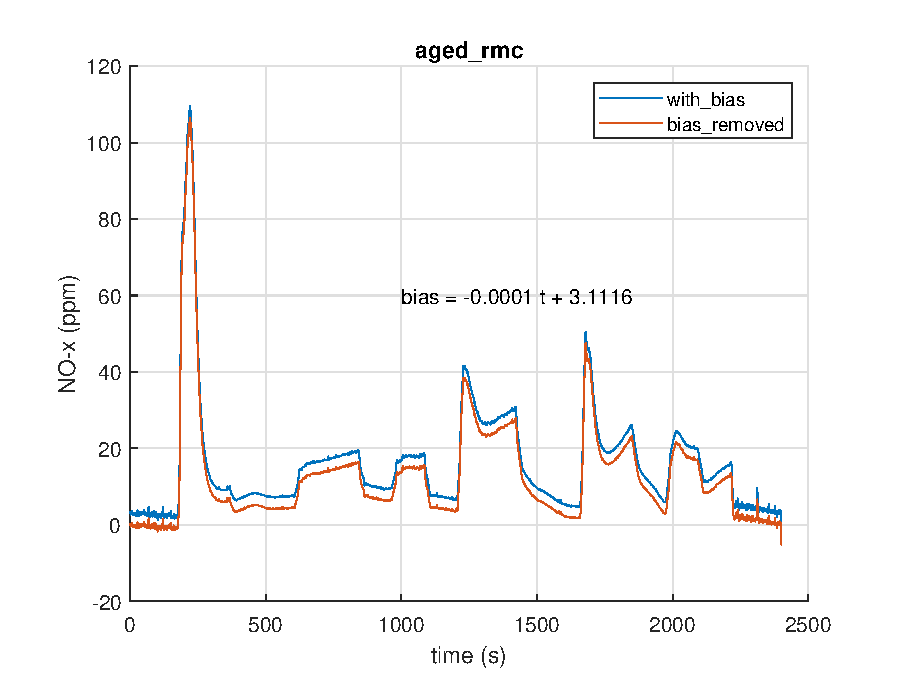
\includegraphics[width=\textwidth]{./figs/chi_est/aged_rmc_NOx_bias.eps}
        \end{figure}
    \end{minipage}
    \begin{minipage}{0.49\textwidth}
        \begin{figure}[H]
            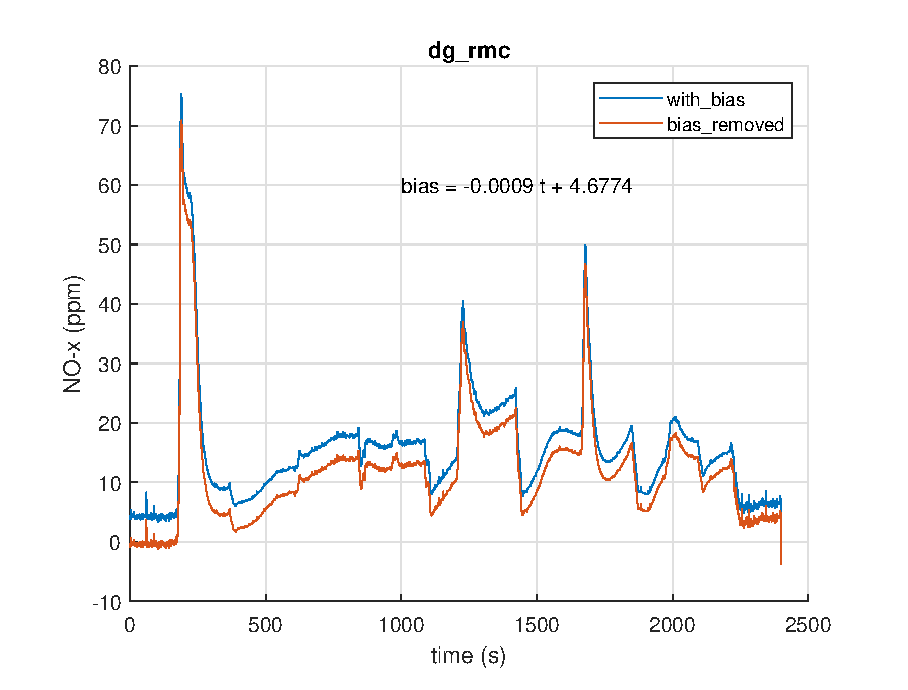
\includegraphics[width=\textwidth]{./figs/chi_est/dg_rmc_NOx_bias.eps}
        \end{figure}
    \end{minipage}
        \caption{Sensor bias correction for RMC cycles}
\end{figure}

\cred{The results depicted above indicate that the coefficient of \( t \), \( b_1 \) (drift), is considerably smaller in comparison to the bias \( b_0 \), suggesting it can be disregarded.}

\subsubsection{Effect of $NH_3$ sensor bias and minimum threshold for cross-sensitivity}
The ammonia sensor used for ammonia measurement also has bias and there is a
threshold on ammonia for which the $NO_x$ sensor becomes cross-sensitive to
ammonia. Thus the expression for cross-sensitivity becomes:

\begin{align*}
    y_1 &= \lr{x_1 - b_0} + \chi (x_2 - b_{th})\\
\end{align*}

\subsubsection{Least-squares estimation assuming temperature independence}
The temperature changes in RMC cycle don't affect the
cross-sensitivity factor significantly. Thus, it can be treated as a constant
w.r.t temperature fluctuations in that range.

We have,
\begin{align*}
    \underbrace{y_1 - x_1}_{\pmb y} &= \underbrace{\bm{x_2 & -1}}_{\pmb \phi^T} \underbrace{\bm{ \chi \\ \underbrace{\chi b_{th} + b_0}_{=b}}}_{ \pmb \theta}\\
\end{align*}

\begin{figure}[H]
    \begin{minipage}{0.49\textwidth}
        \begin{figure}[H]
            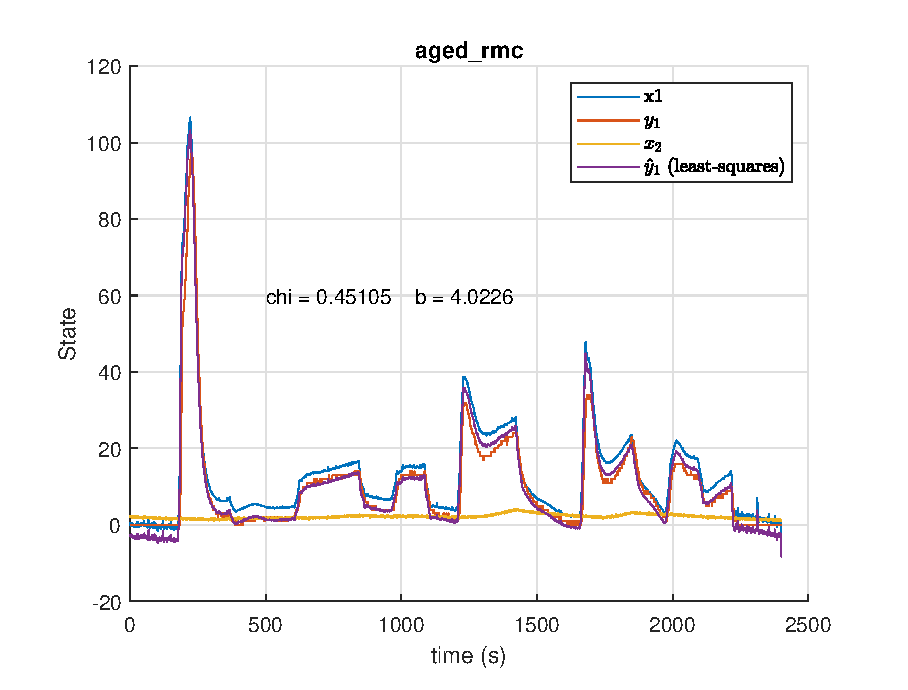
\includegraphics[width=\textwidth]{./figs/chi_est/aged_rmc_chi.eps}
        \end{figure}
    \end{minipage}
    \begin{minipage}{0.49\textwidth}
        \begin{figure}[H]
            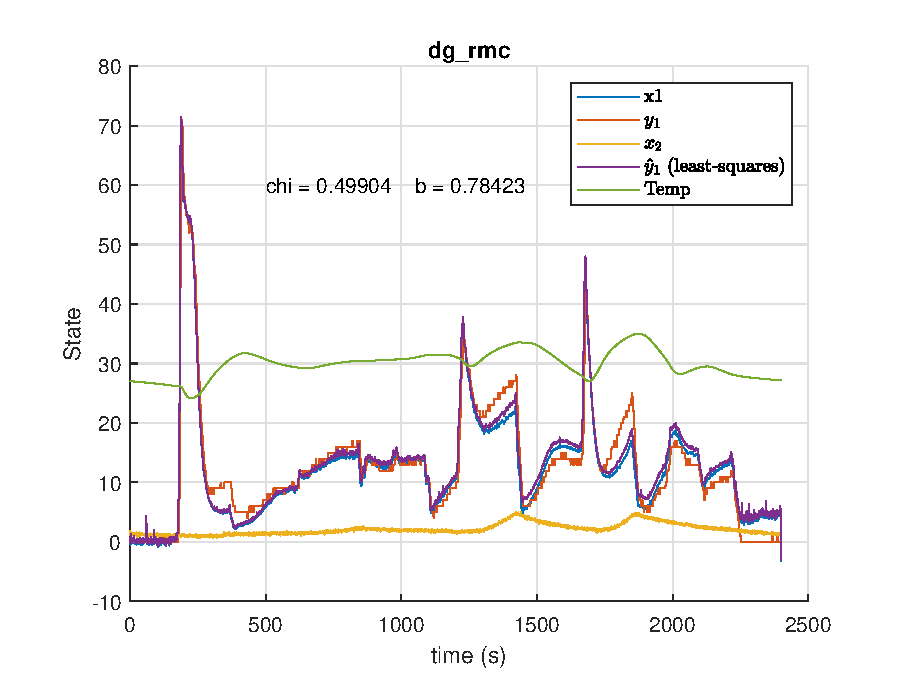
\includegraphics[width=\textwidth]{./figs/chi_est/dg_rmc_chi.eps}
        \end{figure}
    \end{minipage}
        \caption{$\chi$ estimation for RMC cycles}
\end{figure}

\begin{figure}[H]
    \centering
    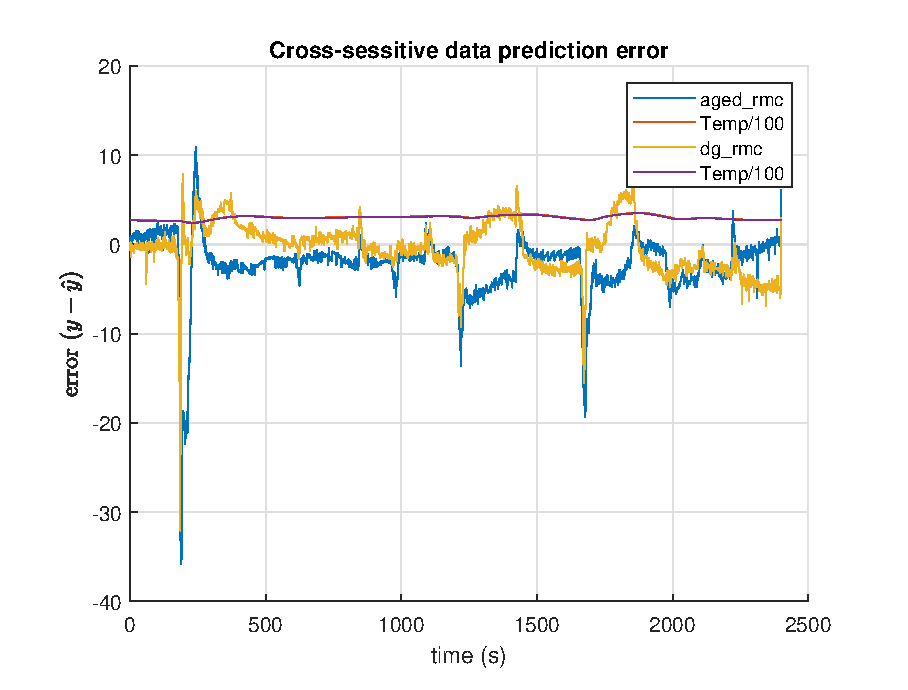
\includegraphics[width = 0.5 \textwidth]{./figs/chi_est/chi_error.eps}
    \caption{Error in $\chi$ estimation}
\end{figure}

The error can be reduced by introducing the effects of temperature into $\chi$.


\subsubsection{Least-squares estimation with $\chi$ as a temperature function}
For simplicity, $\chi$ is assumed to be a linear function of temperature.
\begin{align*}
    \chi(T) &= a T - b_T
\end{align*}

Assuming the sensor-bias is not time-varying ($\because$ $b_1$ is small). The
sensor bias, cross-sensitivity threshold and temperature dependence can be
combined into:

\begin{align*}
    y_1 &=  \lr{x_1 - b_0} + \lr{aT - b_{T}} \lr{x_2 - b_{th}}\\
    \lr{y_1 - x_1} &= a T x_2 - a b_{th} T - b_{T} x_2 + (b_T b_{th} - b_0)\\
    \underbrace{y_1 - x_1}_{\pmb y} &= \underbrace{\bm{T x_2 & -T & -x_2 & 1}}_{\pmb \phi^T} \underbrace{\bm{a \\ a b_{th} \\ b_T \\ b_T b_{th} - b_0}}_{\pmb \theta}\\
\end{align*}

\begin{figure}[H]
    \begin{minipage}{0.49\textwidth}
        \begin{figure}[H]
            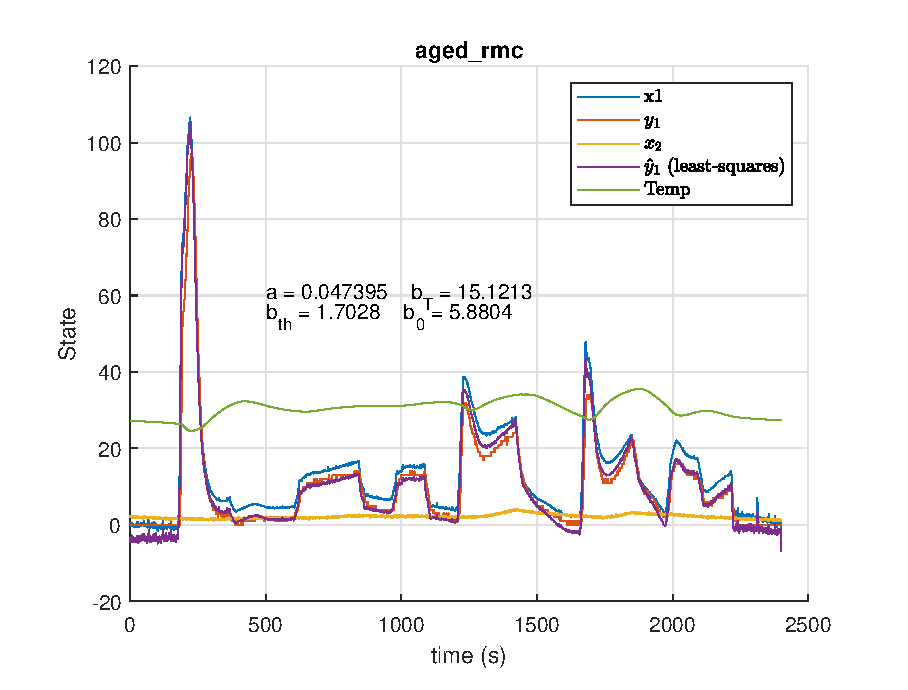
\includegraphics[width=\textwidth]{./figs/chi_est/aged_rmc_chiT.eps}
        \end{figure}
    \end{minipage}
    \begin{minipage}{0.49\textwidth}
        \begin{figure}[H]
            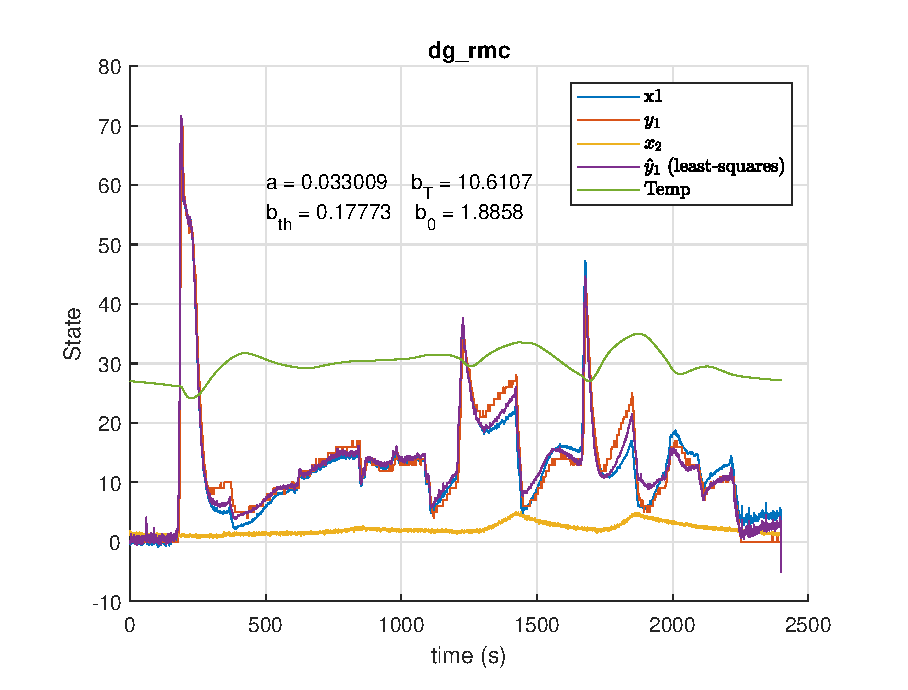
\includegraphics[width=\textwidth]{./figs/chi_est/dg_rmc_chiT.eps}
        \end{figure}
    \end{minipage}
        \caption{$\chi$ estimation for \cred{RMC} cycles}
\end{figure}

\begin{figure}[H]
    \begin{minipage}{0.49\textwidth}
        \begin{figure}[H]
            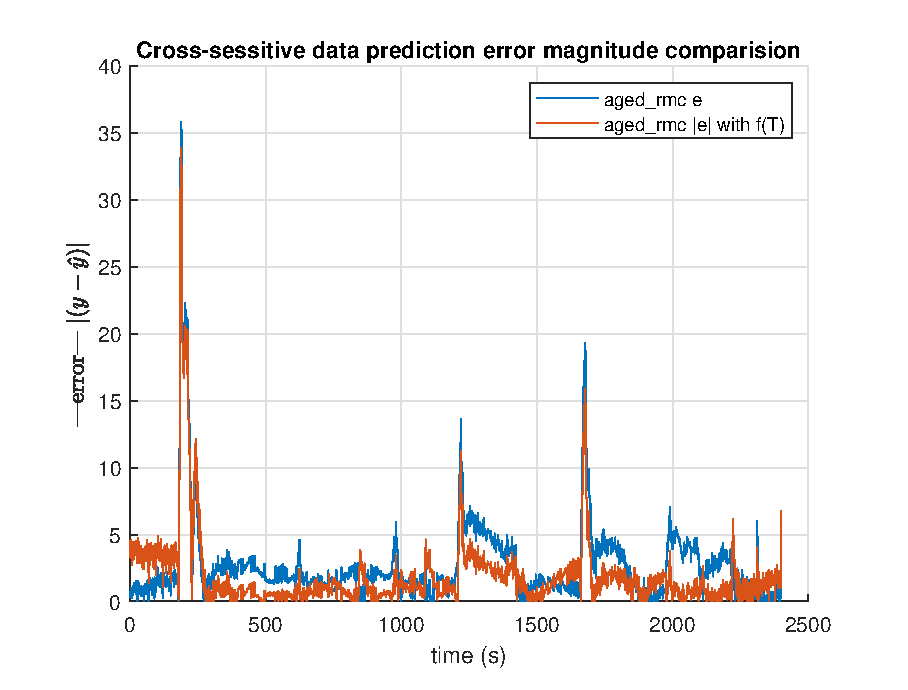
\includegraphics[width=\textwidth]{./figs/chi_est/aged_error_comp.eps}
        \end{figure}
    \end{minipage}
    \begin{minipage}{0.49\textwidth}
        \begin{figure}[H]
            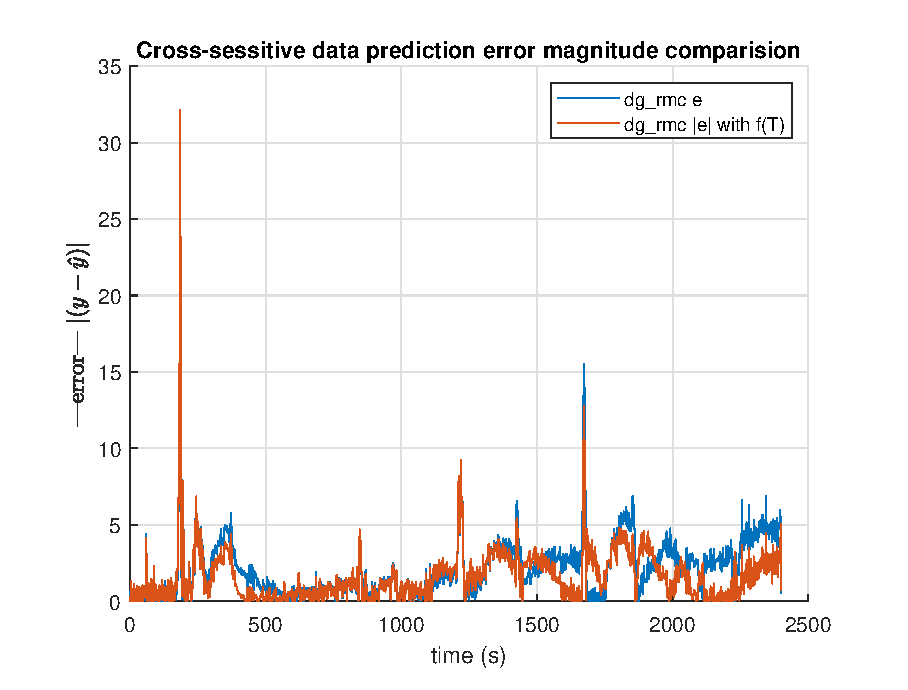
\includegraphics[width=\textwidth]{./figs/chi_est/dg_error_comp.eps}
        \end{figure}
    \end{minipage}
        \caption{Effect of temperature on prediction errors for $\chi$ estimation in RMC cycles}
\end{figure}


Introducing temperature clearly decreases the prediction error in the model. However, the reduction in error, while noticeable, is not significant when compared to the temperature-independent model, whose error remains within acceptable limits.

\section{Catalyst molar storage capacity model}
The variation of storage capacity of the catalyst ($\Theta$) with temperature is
modelled using an exponential curve fit in \cite{hsieh2011development} (2011)
from the available experimental data from
\cite{willems2007closed}, \cite{ciardelli2004scr} and \cite{joo2008study}.  The
results from \cite{schmieg2012thermal} (2012) show a similar trend.

\begin{align*}
    \Theta &= S_1 e^{-S_2 T}
\end{align*}

The parameters $S_1$ and $S_2$ change with age effecting the storage capacity at
a given temperature.

\begin{figure}[H]
    \begin{minipage}{0.49\textwidth}
        \begin{figure}[H]
            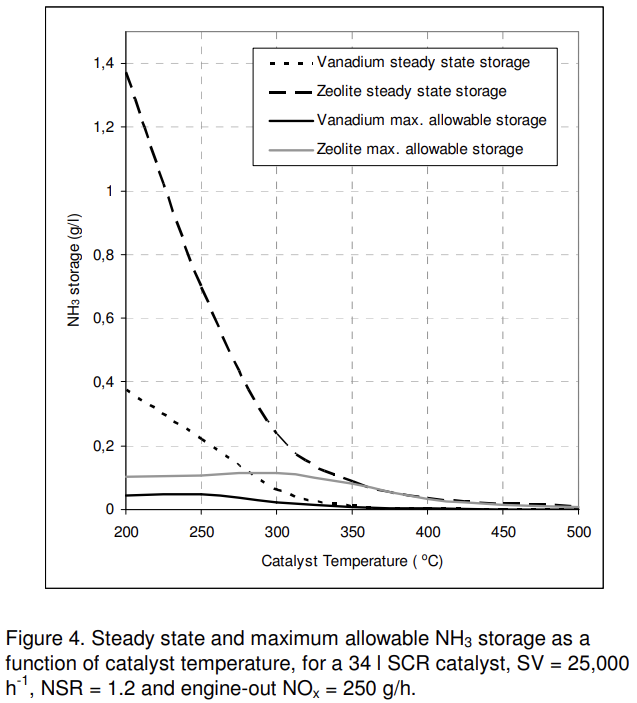
\includegraphics[width = 0.8\textwidth]{./figs/storage_capacity/sae.png}
            \caption*{Results from \cite{willems2007closed}}
        \end{figure}
    \end{minipage}
    \begin{minipage}{0.49\textwidth}
        \begin{figure}[H]
            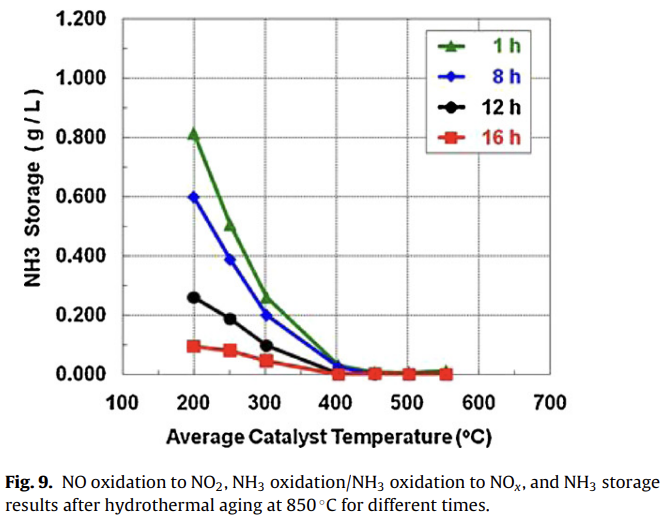
\includegraphics[width = \textwidth]{./figs/storage_capacity/th1.png}
            \caption*{Results from \cite{schmieg2012thermal}}
        \end{figure}
    \end{minipage}
    \begin{minipage}{0.49\textwidth}
        \begin{figure}[H]
            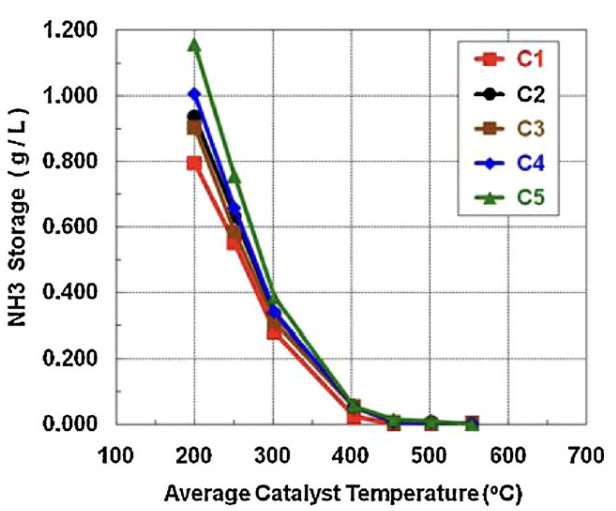
\includegraphics[width = \textwidth]{./figs/storage_capacity/th_2.png}
            \caption*{Results from \cite{schmieg2012thermal}}
        \end{figure}
    \end{minipage}
    \begin{minipage}{0.49\textwidth}
        \begin{figure}[H]
            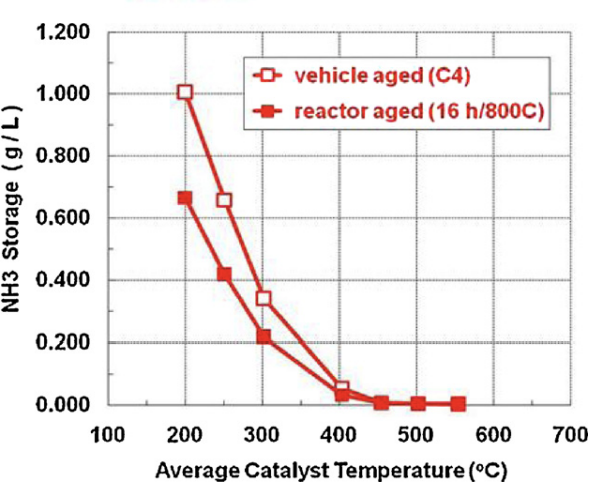
\includegraphics[width = \textwidth]{./figs/storage_capacity/th_3.png}
            \caption*{Results from \cite{schmieg2012thermal}}
        \end{figure}
    \end{minipage}
    \caption{Temperature effects of catalyst storage capacity}
\end{figure}


\input{secs/catalyst_aging_factor.tex}


\subsection{Conclusions}
The full non-linear model for gas concentrations was derived based on a CSTR
model with reduced-order dynamics, that were previously justified in
literature. Model parameters were determined as explicit functions of reaction
rates and the catalyst's ammonia storage capacity.  Parameter identification,
beginning with the output equation and focusing on $NO_x$ sensor
cross-sensitivity ($\chi$), was carried out using RMC test-cell data from
degreened and aged catalysts. A preliminary indicator of aging was observed
from the catalyst's storage capacity versus temperature curve.

\newpage
\section{Research Objectives and Scope}
\subsection{Approach to the research problem}
Our approach is based on the presumption that the aging detection problem can be framed as a state/parameter estimation challenge with respect to the concentration dynamics of the gases involved. This gives rise to the following sub-problems:

\begin{enumerate}
\item Determining a suitable model for the system dynamics.
\item Assessing whether the available data contains sufficient information for identifying the model parameters related to the chosen system dynamics.
\item Investigating the relationship between the parameters/states and the aging factor of the catalyst.
\item Understanding the uncertainties inherent in the aforementioned processes.
\item Finally, developing and validating the aging detection algorithm.
\end{enumerate}

\subsection{Objectives for 2023 (previously)}
\begin{enumerate}
 \item In the current data, the operating conditions in the truck cover a wider range than the ones in test-cell. So, we wish to validate the SCR-ASC model on test-cell data with operating conditions similar to the truck data. If it is difficult to obtain such experimental data in test-cell, then use a high-fidelity SCR-ASC model in AVL Boost, to validate our low fidelity diagnostics-oriented model across a wide range of transient and steady operating conditions.
 \item Explore other low fidelity diagnostics-oriented SCR-ASC model structures, that could be calibrated using the signals between SCR and ASC that could be obtained from the high-fidelity Boost model.
 \item Validate the model-based and data-driven OBD results using truck data from trucks with DG and/or an EUL catalyst.
 \item Validate the model-based and data-driven OBD results using high-fidelity simulations.
 \item Based on the model and OBD validation results, iterate and improve both model-based and data-driven approaches to achieve robust diagnostics performance validated using high-fidelity simulations and actual data. Also implement a more rigorous and detailed version of the stochastic model-based OBD.
 \item Support TTU in development and demonstration of model-based, data-driven, and frequency-domain OBD methods that rely on detecting NOx-rich regions where ASC is inactive.
\end{enumerate}


\subsection{Objectives for 2024}
\begin{enumerate}
\item Identify the model parameters and parametric uncertainties using
the test-cell data and data from AVL boost model and validate them.
\item Develop the estimation methodology for the storage capacity (Observer Design).
\item Relate catalyst's aging to the storage capacity and develop robust
non-intrusive aging detection algorithm and test the algorithm on the test-cell
data and the road data segments.
\end{enumerate}
\subsection{Objectives post-2024}
\begin{enumerate}
    \item Provide an assessment of the potential to embed the algorithms in a real-time system.
    \item Implementation and comprehensive evaluation, including robustness analysis, of the proposed diagnostic algorithms in engine test cell and on the road.
\end{enumerate}


\subsection{Other requirements}
\begin{itemize}
    \item Prior to the end of this project, a proposal for follow-on work will be submitted to Cummins.
    \item Cummins to provide expertise via mentorship and regular feedback.
    \item Cummins to provide funds to support the students.
    \item Cummins to provide test-cell data with operating conditions similar to on-road trucks
    \item Cummins to provide truck data with at least one and preferably two known aging levels (could be DG and/or EUL)
    \item Cummins to provide access to high-fidelity AVL Boost model for SCR-ASC. This could be a black-box model with access to pre-SCR, post-SCR, post-ASC signals, and NH3 storage values in SCR and ASC.
\end{itemize}

\section{Intellectual Property}
(Select)
\begin{itemize}
    \item Track 1 - CNERF (8.4.1)
    \item Track 2 - 5-Year Exclusive License (8.4.2)
    \item Track 3 - Work-for-Hire - IP Assignment (8.4.3)
\end{itemize}

\section{Publication}
{\color{red}(Select)}
\begin{itemize}
    \item  Publication Review
    \item Publication Approval (Requires Purdue Export Control Technology Control Plan) (8.6.3)
\end{itemize}

\section{Timeline and Deliverables}
\subsection{Timeline for 2024}

\begin{table}[H]
    \centering
    \begin{tabular}{l l l}
        \hline\hline
                & Task & $|$Quarter1$|$Quarter2$|$Quarter3$|$Quarter4$|$ \\\hline\hline
        1.      & Model parameter identification   & $|++++|----|----|----|$\\
        2.      & Validating identified model      & $|--++|++--|----|----|$\\
        3.      & Formal definition of aging factor& $|----|--++|----|----|$\\
        4.      & Algorithm development            & $|----|----|++++|++--|$\\
        5.      & Validation                       & $|----|----|----|++++|$\\
        \hline\hline
    \end{tabular}
\end{table}
\subsection{Deliverables}
The deliverables for the research project will be in the form of documentation
and the code for processing data and validation of algorithms.

\begin{enumerate}
    \item The documentation includes:
\begin{enumerate}
    \item Detailed system model derived from the first principles with assumptions.
    \item Model parameter estimation methods and the results of such endeavor.
    \item Formal definition of aging factor estimation problem.
    \item Aging factor estimation algorithm and validation results.
\end{enumerate}

\item The code repository will include routines for:
\begin{enumerate}
    \item Model parameter estimation and validation using test-cell data.
\item Programs for handling the AVL boost simulation model provided for model
parameter identification purposes.
\item Aging factor estimation for test-cell and truck data and validation using
test-cell data.
\end{enumerate}

\end{enumerate}

\section{Budget}

\begin{table}[H]
    \centering
    \begin{tabular}{r r}
    \hline \hline
    Line Item           & Year 2024 \\ \hline \hline
    \textit{Personnel Costs}&\\
    Faculty Salaries:   & $\$ 19,635.03$\\
    Student Salaries:   & $\$ 35,886.41$\\
    Grad Remission Fee: & $\$ 11,180.04$\\
    \hline
	Travel:             & $\$  4,000.00$\\
    S$\&$E:             & $\$  1,000.00$\\
    Indirect Costs:     & $\$ 34,497.22$\\ \hline
    \bf{Total}:              & $\$ 106198.70$\\
    IP Fees:            & $\$ 10,619.87$\\ \hline \hline
    \itbf{Grand Total}:       & $\$ 116,818.57$\\
    \hline \hline
    \end{tabular}
\end{table}
\begin{flushright}
\end{flushright}

Cummins will generate a quarterly PO for each quarter of the approved Research
Project Plan to facilitate quarterly payments provided at the beginning of each
project quarter.\\

\noindent \textbf{PURDUE RESEARCHER}: Prof. Peter H. Meckl\\

\noindent \textbf{CUMMINS PRINCIPAL INVESTIGATOR}: Lyle E. Kocher\\


\noindent \itbf{By signing below, the parties authorized representatives agree to this Research Project Plan.}

\begin{table}[H]
    \centering
    \begin{tabular}{l c l}
        \itbf{CUMMINS, INC.} & $\qquad$ &\itbf{PURDUE UNIVERSITY}\\
        By:$\_\_\_\_\_\_\_\_\_\_\_\_\_\_\_\_\_\_\_\_\_\_\_\_\_\_\_\_\_$ & $\qquad$ &
        By:$\_\_\_\_\_\_\_\_\_\_\_\_\_\_\_\_\_\_\_\_\_\_\_\_\_\_\_\_\_$ \\
        Printed Name : & $\qquad$ & Printed Name:\\
Title:$\_\_\_\_\_\_\_\_\_\_\_\_\_\_\_\_\_\_\_\_\_\_\_\_\_\_\_\_\_$ &	$\qquad$
&Title:
                $\_\_\_\_\_\_\_\_\_\_\_\_\_\_\_\_\_\_\_\_\_\_\_\_\_\_\_\_\_$ \\
Date: $\_\_\_\_\_\_\_\_\_\_\_\_\_\_\_\_\_\_\_\_\_\_\_\_\_\_\_\_\_$ & $\qquad$ &
Date: $\_\_\_\_\_\_\_\_\_\_\_\_\_\_\_\_\_\_\_\_\_\_\_\_\_\_\_\_\_$\\
    \end{tabular}
\end{table}



\newpage
\bibliographystyle{unsrt}
\bibliography{refs}

%===============================================================================
\newpage
\begin{

\newpage
%===============================================================================
\begin{center}
    APPENDIX C\\
    \bigskip
    ASSIGNMENT
\end{center}

\end{document}
